% !TEX root = paper/paper.tex
\section{Learning the policy}
We seek a policy $\pi$ that maximizes the expected value of the MDP, so actions should be selected proportionally to their expected value.
Specifically, we want
\begin{equation*}
\argmax_a \pi(a \mid s) = \argmax_a Q(s,a)
\end{equation*}
where $Q(s,a)$ is the \emph{action-value function}, which is defined analogously to the value function \eqref{eq:expected_reward}.
(See \cite{Sutton1998} for a thorough review of MDPs and reinforcement learning techniques.)

However, the dimensionality of information that has to be encoded in the state forbids an exact representation of $Q(s,a)$.
Instead, we use feature approximation and write $Q(s,a) = \theta^T \phi(s, a)$,  where $\phi: \mathcal{S} \times \mathcal{A} \mapsto \mathbb{R}^{d_s}$ is the featurization function, $d_s$ is the dimensionality of the state feature vector, and $\theta$ is a vector of weights that defines the policy.

Specifically, the policy is defined as
\begin{equation}
\pi(a \mid s) = \frac{\exp\left(\frac{1}{\tau} \theta^T \phi(s, a)\right)}{\sum\limits_{a' \in \mathcal{A}} \exp\left(\frac{1}{\tau} \theta^T \phi(s, a')\right)}
\end{equation}
where $\tau$ is a temperature parameter that controls the level of exploration vs. exploitation in the policy.
As $\tau \rightarrow 0$, ${\pi(a \mid s)}$ becomes highly peaked at $\argmax_a Q(s,a)$; it becomes uniform as $\tau \rightarrow \infty$.

\subsection{State feature vector.} \label{sec:policy_features}

The function $\phi(s)$ extracts the following features from the state:

\begin{itemize}
\item Bit vector of length $F$ representing whether the corresponding feature has been computed or not; initially $0$.
\item For each $h_f$, a vector of size $d_f$ representing the values; $0$ until computed.
\item Cost feature $c \in [0, 1]$ for fraction of the budget spent.
\item Bias feature $1$.
\end{itemize}

The state-action feature function $\phi(s, a)$ block-codes these features: it is $0$ everywhere except the block corresponding to the action considered.

\paragraph{Dynamic vs. Static State.}
These features define the \textbf{dynamic} state, presenting enough information to have a \emph{closed-loop} (dynamic) policy that may select different features for different test instances.

The \textbf{static} state has all of the above features except for the observed feature values.
This enables only an \emph{open-loop} (static) policy, which is exactly the same for all instances.
Policy learned with the static state is used as a baseline in experiments.

\subsection{Computing rewards and state-action values.} \label{sec:rewards}
In the \hyperref[def:MDP]{MDP definition}, we noted that the reward function is specified manually.
Recall that each step of the sequential feature selection $\pi$ adds a feature to the subset of computed features, which can be combined by $\rho$ to give the answer $g(x)$.

\paragraph{Final vs. Anytime performance.}
We strive for best performance under $\mathcal{G}_\mathcal{B}$, which can be defined in one of two ways:
(a) only the \textbf{final} answer $g(x)$ with cost $C_{g(x)} \leq \mathcal{B}$ is evaluated;
or (b) $g(x)$ is evaluated after every feature computation, with the goal of \textbf{\emph{Anytime}} performance.
In the following, we consider the \emph{Anytime} case, which is motivated by settings where feature selection may be arbitrarily stopped before the budget runs out fully.

\paragraph{}
Consider \hyperref[fig:rewards]{Figure~\ref*{fig:rewards}}, which shows the entropy of $\Rho$ and the 0-1 loss of $\rho$ at every point in a sequential feature selection episode.
For the best \emph{Anytime} performance, we want to capture the most area above the loss vs. cost curve.
Recall from \eqref{eq:expected_reward} that the value of an episode $\xi$ is defined as the sum of obtained rewards.
If the reward of a single action is defined as the area above the curve that is captured as a direct result, then the value of the whole episode exactly corresponds to $\mathcal{G}_\mathcal{B}$.

But there is a problem with using this definition of the reward function: all actions after the first would have 0 reward, as they do not decrease the loss any further.
Further, although $\rho$ is tipped toward the correct classification after the first action, it remains quite uncertain in its answer.

Because we aim to decrease uncertainty and would like the reward function to be smooth and not discontinuous, we define the reward as the area above the entropy vs. cost curve.
\hyperref[fig:rewards]{Figure~\ref*{fig:rewards}} provides the precise definition.

\begin{figure}[t]
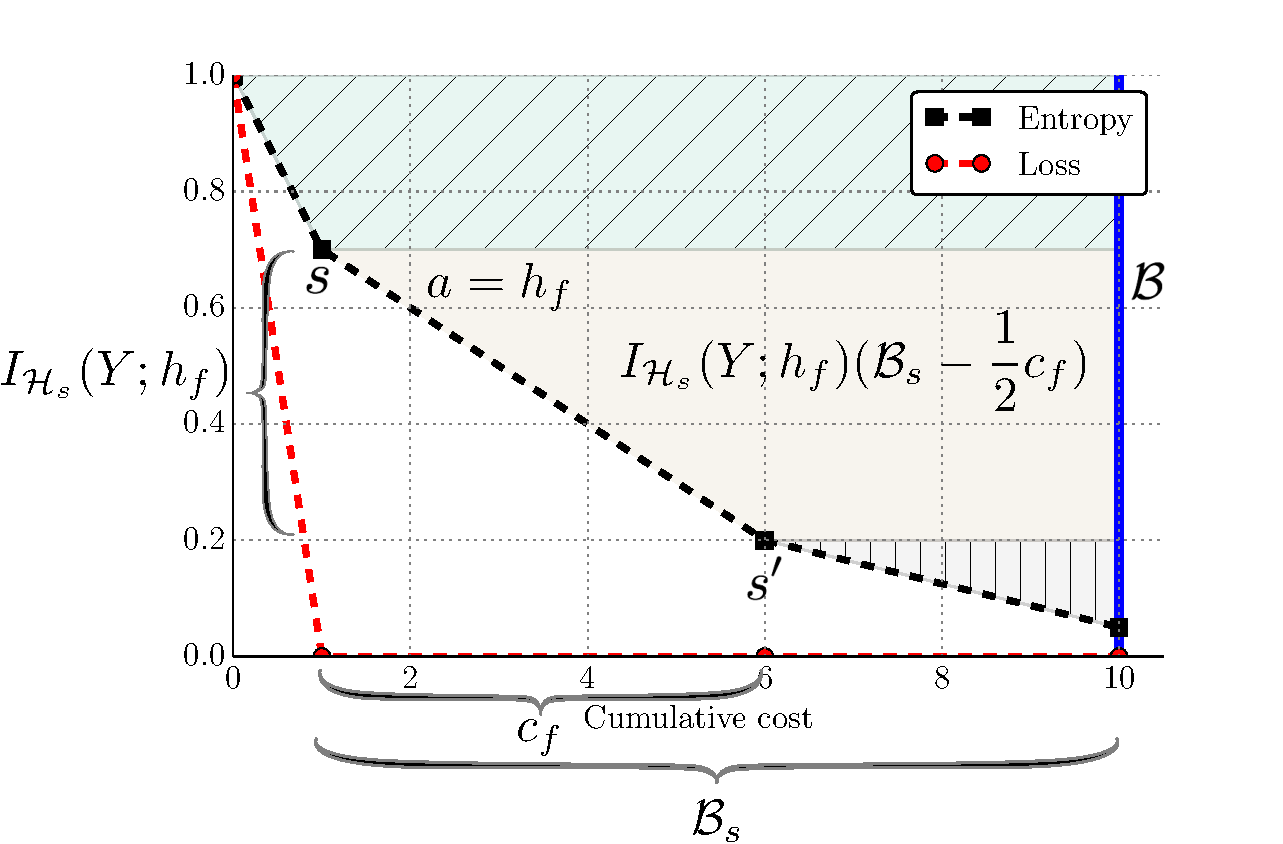
\includegraphics[width=1\linewidth]{../../figures/rewards}
\caption{Definition of the reward function.
We seek to maximize the total area above the entropy vs. cost curve from $0$ to $\mathcal{B}$, and so define the reward of an individual action as the area of the slice of the total area that it contributes.
From state $s$, action $h$ leads to state $s'$, with corresponding cumulative costs $s_c$ and $s_c'$.
${I(\Rho; h) = -\left[ H(\Rho_{s'}) - H(\Rho_s) \right]}$ is the \emph{information gain} of $h$.}
\label{fig:rewards}
\end{figure}

\todo{Evaluate both reward settings!}

\paragraph{Greedy vs. Undiscounted Value.}
The $\gamma$ parameter of the MDP controls the level of \emph{discounting} of rewards of future action in computing the value \eqref{eq:expected_reward}.
In the baseline \textbf{greedy} setting, with $\gamma=0$, rewards gained by future actions are not counted at all in determining the value of the current action.
In the \textbf{undiscounted}, with $\gamma=1$, rewards gained by future actions are valued exactly as much as reward gained by the current action in determining its value.
The latter setting is used as a baseline.

\subsection{Learning method.}
Given the state feature vector and the computed rewards, we need to learn a predictor for rewards of future states.

The policies are parametrized by $\theta$ and $\tau$, but only $\theta$ is a learned parameter.
At test time, $\tau$ is set to a value close to $0$ to make the policy essentially deterministic.
During training, it is gradually lowered from a high value to ensure sufficient exploration of the state space.

\paragraph{Random.}
We first consider a baseline policy that selects features completely randomly (although no feature is selected more than once).
No learning at all is needed for this policy.

\paragraph{Linear Regression.}
Because we can compute the exact value $Q(s,a)$ for any $s,a$ that we see in training, $\theta$ can be learned by minimizing error between $\theta^T \phi(s,a)$ and the actual computed value (remember that $Q(s,a) = \theta^T \phi(s,a)$).
We implement this with $L_2$-regularized regression.

Instead of block-coding $\phi(s,a)$, we learn $F$ separate $\theta_f$'s for the features $\phi(s)$: one for each action $a$.
The weight $\alpha$ of the regularization term is tied across the $F$ separate regressions and is tuned by cross-validation on 3 folds.

\paragraph{Policy Gradient.}
\todo{
    We can also use the \emph{policy gradient} method of learning the policy.
    It's unlikely to work better and will be slower, so I've been reluctant to implement it, but it's something that could be done fairly easily.
}
% With our parametrization of $\pi$, we can rewrite \eqref{eq:expected_reward} as $V_\theta(s) = \mathbb{E}_{p(\xi \mid \theta, x)} r(\xi)$ where $p(\xi \mid \theta, x)$ can be decomposed into a product over time steps:
% \begin{equation*}
% p(\xi \mid \theta, x) = \prod_{t=0}^{T-1} \pi_\theta(a \mid s_t) \, T_x(s_{t+1} \mid s_t, a)
% \end{equation*}

% The gradient is given by
% \begin{equation} \label{eq:complete_derivative}
% \pder{\theta} V_\theta(s) = \mathbb{E}_{p(\xi \mid \theta, x)} \left[ r(\xi) \sum_t \pder{\theta} \log \pi_\theta(a_t \mid s_t) \right]
% \end{equation}

% The inner partial derivative is given by:
% \begin{equation}
% \pder{\theta} \log \pi_\theta(a_t \mid s_t) = \phi(s,a) - \sum_{a' \in \mathcal{A}} \phi(s, a') \pi_\theta(a' \mid s)
% \end{equation}

% The complete derivative of \eqref{eq:complete_derivative} is intractable due to the infinite number of possible histories.
% Instead, we follow the \emph{policy gradient} method \cite{Sutton-NIPS-2000} and estimate the expectation by sampling trajectories $\xi$, as shown in \hyperref[alg:learning]{Algorithm \ref*{alg:learning}}.